\documentclass{standalone}

\usepackage{pgfplots}

%% Color Settings
\usepackage{xcolor}
\definecolor{iftucfont}{RGB}{74,130,70}
\definecolor{iftuccolor}{RGB}{143,168,92}
\definecolor{iftucbackground}{RGB}{241,244,234}


\pgfplotsset{%
	colormap={whitered}{color(0cm)=(white);
		color(1cm)=(iftuccolor)}
}
\begin{document}
	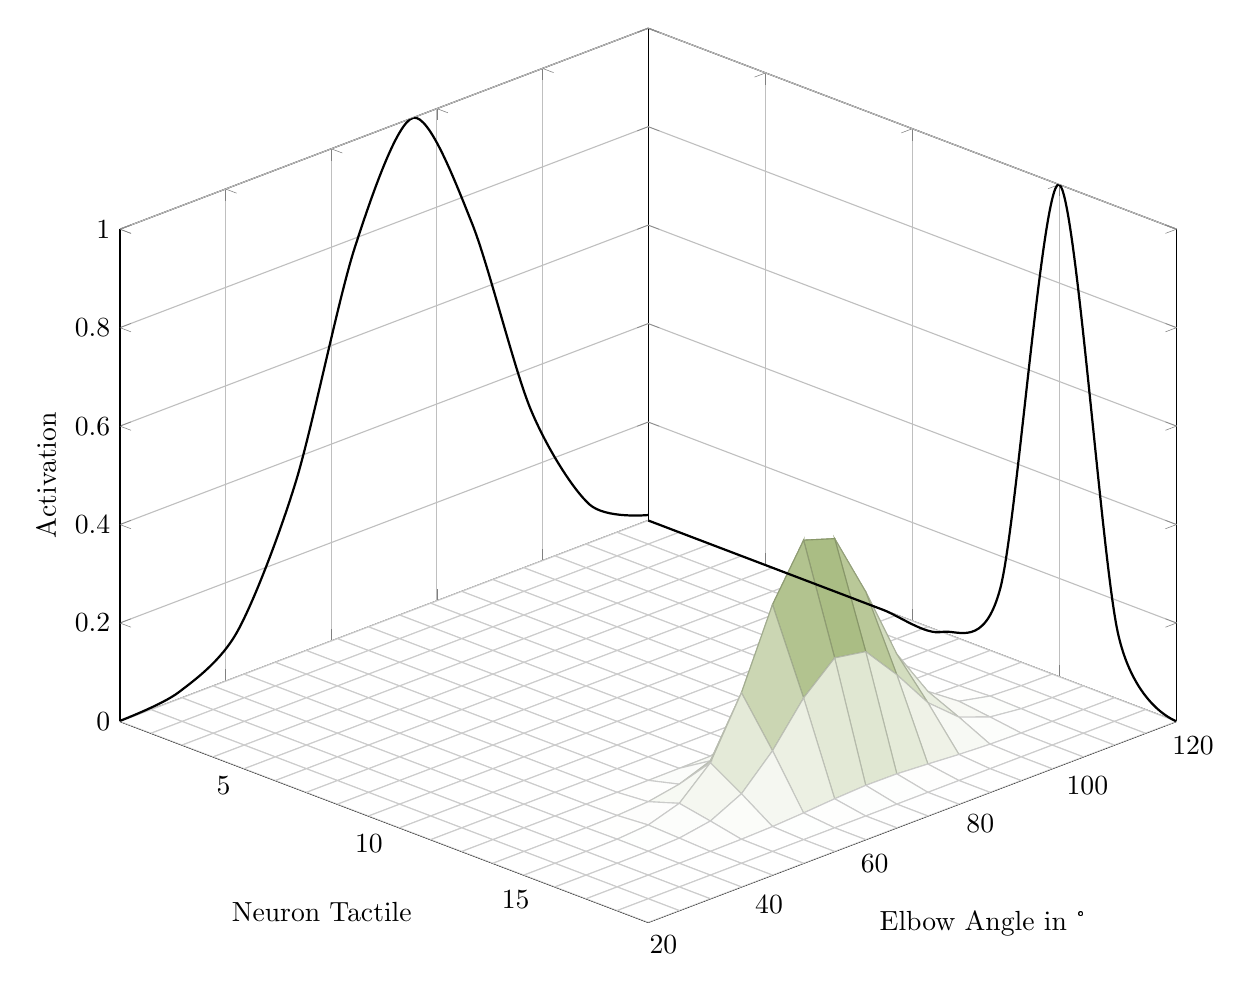
\begin{tikzpicture}[
		declare function = {mu1=15;},
		declare function = {mu2=75;},
		declare function = {sigma1=1;},
		declare function = {sigma2=15;},
		declare function = {normal(\m,\s)=exp(-(x-\m)^2/(2*\s^2));},
		declare function = {bivar(\ma,\sa,\mb,\sb)=
			exp(-((x-\ma)^2/\sa^2 + (y-\mb)^2/\sb^2))/2;}]
		\begin{axis}[
			colormap name  = whitered,
			width          = 15cm,
			view           = {45}{30},
			enlargelimits  = false,
			grid           = major,
			domain         = 1:19,
			y domain       = 20:120,
			samples        = 18,
			xlabel         = Neuron Tactile,
			ylabel         = Elbow Angle in °,
			zlabel         = {Activation}
			]
			\addplot3 [surf] {bivar(mu1,sigma1,mu2,sigma2)};
			\addplot3 [domain=1:19,samples=10, samples y=1, thick, smooth]
			(x,120,{normal(mu1,sigma1)});
			\addplot3 [domain=20:120,samples=10, samples y=1, thick, smooth]
			(1,x,{normal(mu2,sigma2)});
			
		\end{axis}
	\end{tikzpicture}
\end{document}